
\documentclass[16pt]{report}
\usepackage[portrait, top=3cm, bottom=2cm, left=3cm, right=3cm]{geometry}

\usepackage{cancel}
\usepackage{hyperref}
\usepackage[labelformat=empty]{caption}
\usepackage[utf8]{inputenc}
\usepackage{hyperref}
\usepackage[english,russian]{babel}
\usepackage{listings}
\usepackage[dvipsnames]{xcolor}
\usepackage{setspace}
\usepackage[shortlabels]{enumitem}
\hypersetup{
    colorlinks=true,
    linkcolor=blue,
    filecolor=blue,      
    urlcolor=blue,
}

\usepackage{amsmath,amsfonts,amssymb,amsthm,mathtools} 
\usepackage[usenames,dvipsnames,svgnames,table]{xcolor}
\usepackage{lettrine} %%% To make a Drop Cap
\usepackage{yfonts} %% to make a fancy Gothic drop caps.
\usepackage{amsfonts}
\usepackage{wasysym}
\usepackage{tikz}
\usetikzlibrary{arrows, automata, positioning}
\usepackage{colortbl}
\usepackage{lastpage}



\title{DSP HW2}
\author{Dmitrii Masnyi}
\date{November 2021}

\begin{document}

\maketitle
\section*{Task 1}
Design a low pass FIR filter with parameters: passband Fpass = 5 MHz; stopband Fstop = 6MHz; attenuation at least 60 dB in the stopband (out-of-band attenuation). \\
Let the sampling frequency be Fs = 50 MHz.\\
Determine the design with the lowest computational complexity. \\ 
Provide code. \\ \\
\textbf{Solution:} 
\begin{itemize}
\item\textbf{Fir1 filter} \\
First of all, I tried to implement fir1 filter. Because I need to guarantee out-of-band attenuation at least 60 dB I used Blackman window (I tried to implement Hamming window but its attenuation was not sufficient enough). I just ran multiple times the function \textbf{fir1()} with different parameter n and choose \textbf{n} that gave me results that is specified in the problem statement. Finally, I designed fir1 filter with \textbf{n = 300}, which satisfies requirements.
\begin{figure}[h!]
    \center{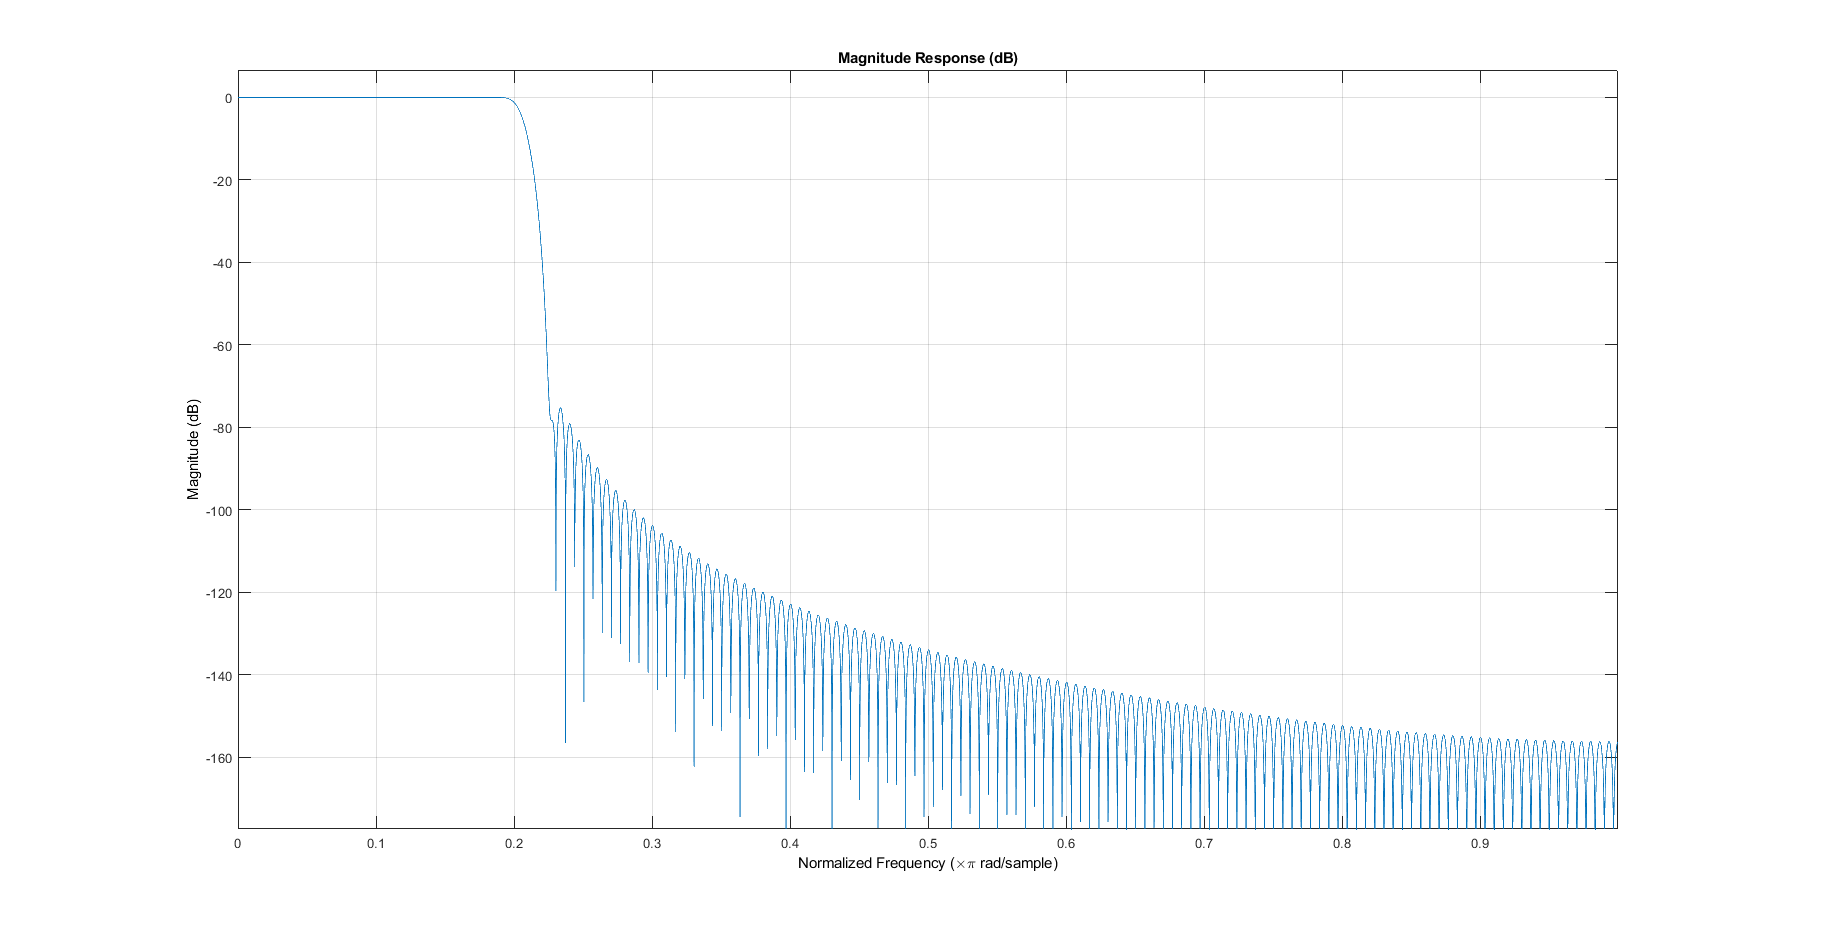
\includegraphics[scale=0.35]{Task1_fir1_blackman.png}}
    \caption{Figure 1: Magnitude response of fir1 filter with blackman window and n = 300.}
    \label{fig:my_label}
\end{figure}
\item\textbf{Fir2 filter}
Then I designed fir2 filter. I used function \textbf{fir2()} and ran it multiple with different parameter \textbf{n} and chose \textbf{n=210}, because fir2 with this parameter satisfies requirements.
\begin{figure}[h!]
    \center{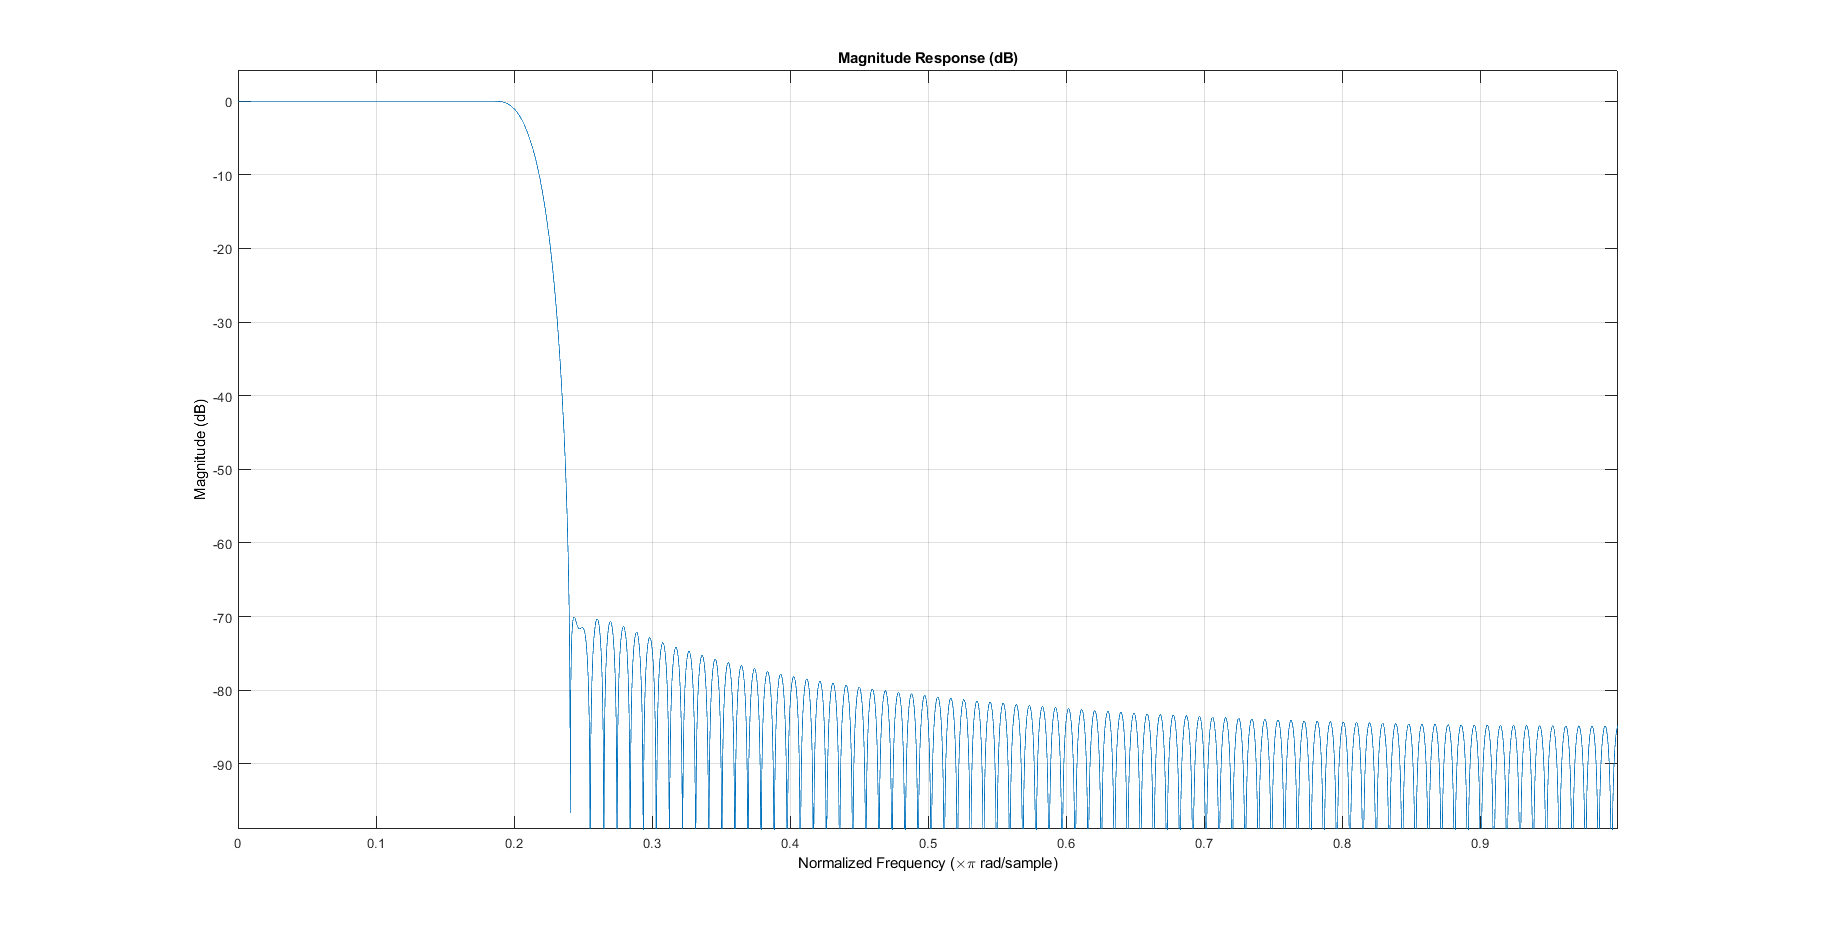
\includegraphics[scale=0.35]{Task1_fir2.png}}
    \caption{Figure 2: Magnitude response of fir2 filter with n = 210.}
    \label{fig:my_label}
\end{figure}
\newpage
\item\textbf{Firls filter} \\
Then I designed firls filter. I used function \textbf{firls()} and ran it multiple times with different parameter \textbf{n} and chose \textbf{n=185}, because firls with this parameter satisfies requirements.
\begin{figure}[h!]
    \center{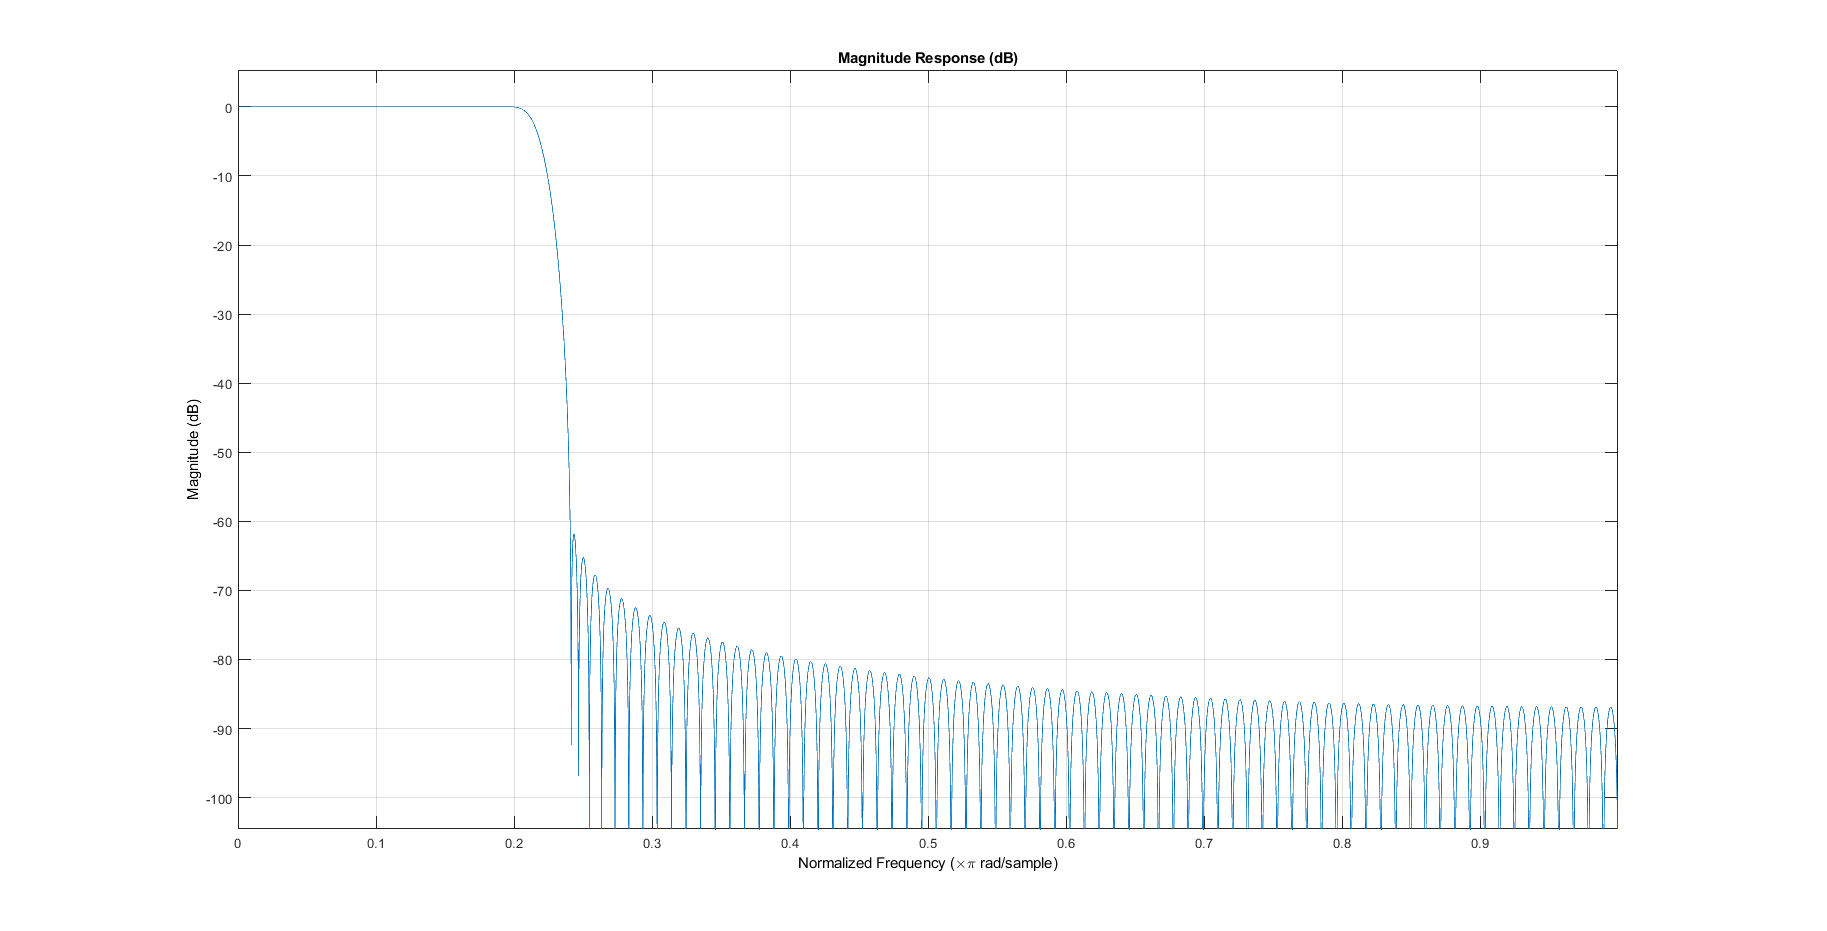
\includegraphics[scale=0.35]{Task1_firls.png}}
    \caption{Figure 3: Magnitude response of firls filter with n = 185.}
    \label{fig:my_label}
\end{figure}
\end{itemize}
\newpage
\begin{lstlisting}
Fpass = 5e6;
Fstop = 6e6;
Fs = 50e6;
%fir1
n = 300;
delta = 0.007; % because default attenuation in wpass = -6dB, so I need to 
%shift magn. resp.
f1 = fir1(n, 2 * Fpass / Fs + delta, blackman(n + 1));
%fvtool(f1);
%fir2
delta = 0.01;
freq = [0 2*Fpass/Fs (2*Fstop/Fs - delta) 1]; % substruction delta is necessary 
%for the proper filter design
mag = [1 1 0 0];
n = 210;
f2 = fir2(n, freq, mag);
%fvtool(f2);
%fir ls
freq = [0 2*Fpass/Fs 2*Fstop/Fs  1]; 
mag = [1 1 0 0];
n = 185;
f3 = firls(n, freq, mag);
fvtool(f3);
\end{lstlisting}
So the filter with the lowest complexity is the firls filter, because it has the least order (\textbf{n = 185}).

\section*{Task 2}
Using the impulse invariance method for analog to digital filter conversion, calculate the Cebyshev lowpass digital filter with parametrers: passband 20MHz; passband ripple 0.2 dB; stopband (out-of-band) attenuation 60 dB; sampling frequency Fs = 100 MHz.\\
a) Plot the impulse response for both analog and digital systems. \\
b) Plot the magnitude response for analog and digital systems in the frequency domain. \\
Provide code. \\ \\
\textbf{Solution:} \\
First of all, I need to design Chebyshev type I analog filter, then using impulse invariance approximation design the digital prototype of the analog Chebyshev type I filter. \\ \\
Matlab has a lot of built-in functions for digital filter designing. For this task I will use \textbf{cheby1(n, Rp, Fpass, 's')} function, which requires these parameters: \\
\begin{itemize}
    \item n - the order of the filter;
    \item Rp - passband ripple;
    \item Wp - passband;
\end{itemize}
Before using this function I need to calculate the order of the filter which I want to design. I will use a built-in Matlab function \textbf{cheb1ord(Wp,Ws,Rp,Rs)}, which returns the order of the filter n.
\begin{itemize}
    \item Wp - passband frequency;
    \item Ws - stopband frquency;
    \item Rp - passband ripple;
    \item Rs - stopband attenuation;
\end{itemize}
Note that stopband frequency is not specified in this task, so I will specify it by myself. Of course, this parameter affects on the complexity on the filter: the narrower the transition band, the more complex the filter. I ran the function \textbf{cheb1ord(Wp,Ws,Rp,Rs)} with different parameter \textbf{Ws} and received this results: 
\begin{itemize}
    \item Ws = 21 MHz, n = 25;
    \item Ws = 25 MHz, n = 11;
    \item Ws = 30 MHz, n = 8;
\end{itemize}
Indeed, the narrower the transition band, the higher n. So, let's choose Ws = 25 MHz. Then n = 11. The next computation will be done for the parameters \textbf{Ws = 25 MHz}, \textbf{n = 11}. Then by writing simple Matlab code I received:

\begin{figure}[h!]
    \center{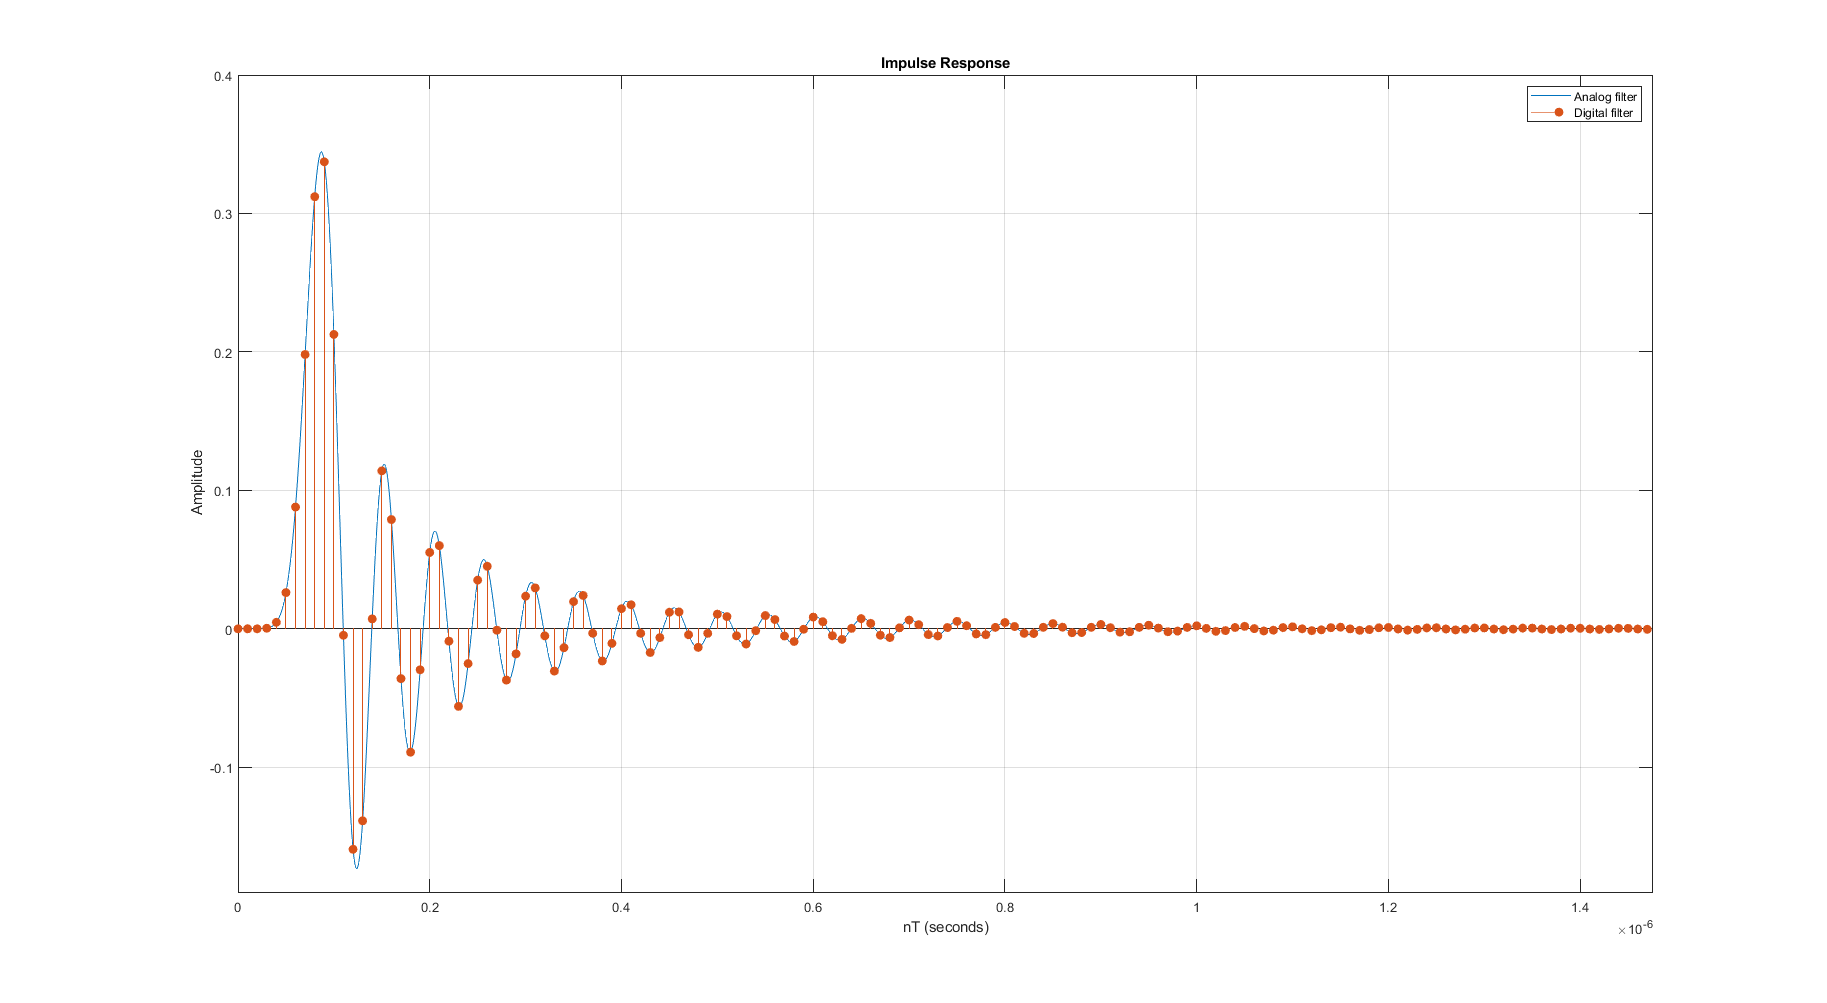
\includegraphics[scale=0.35]{Task2_IR.png}}
    \caption{Figure 4: Impulse response of the analog and the digital filters.}
    \label{fig:my_label}
\end{figure}
\begin{figure}
    \center{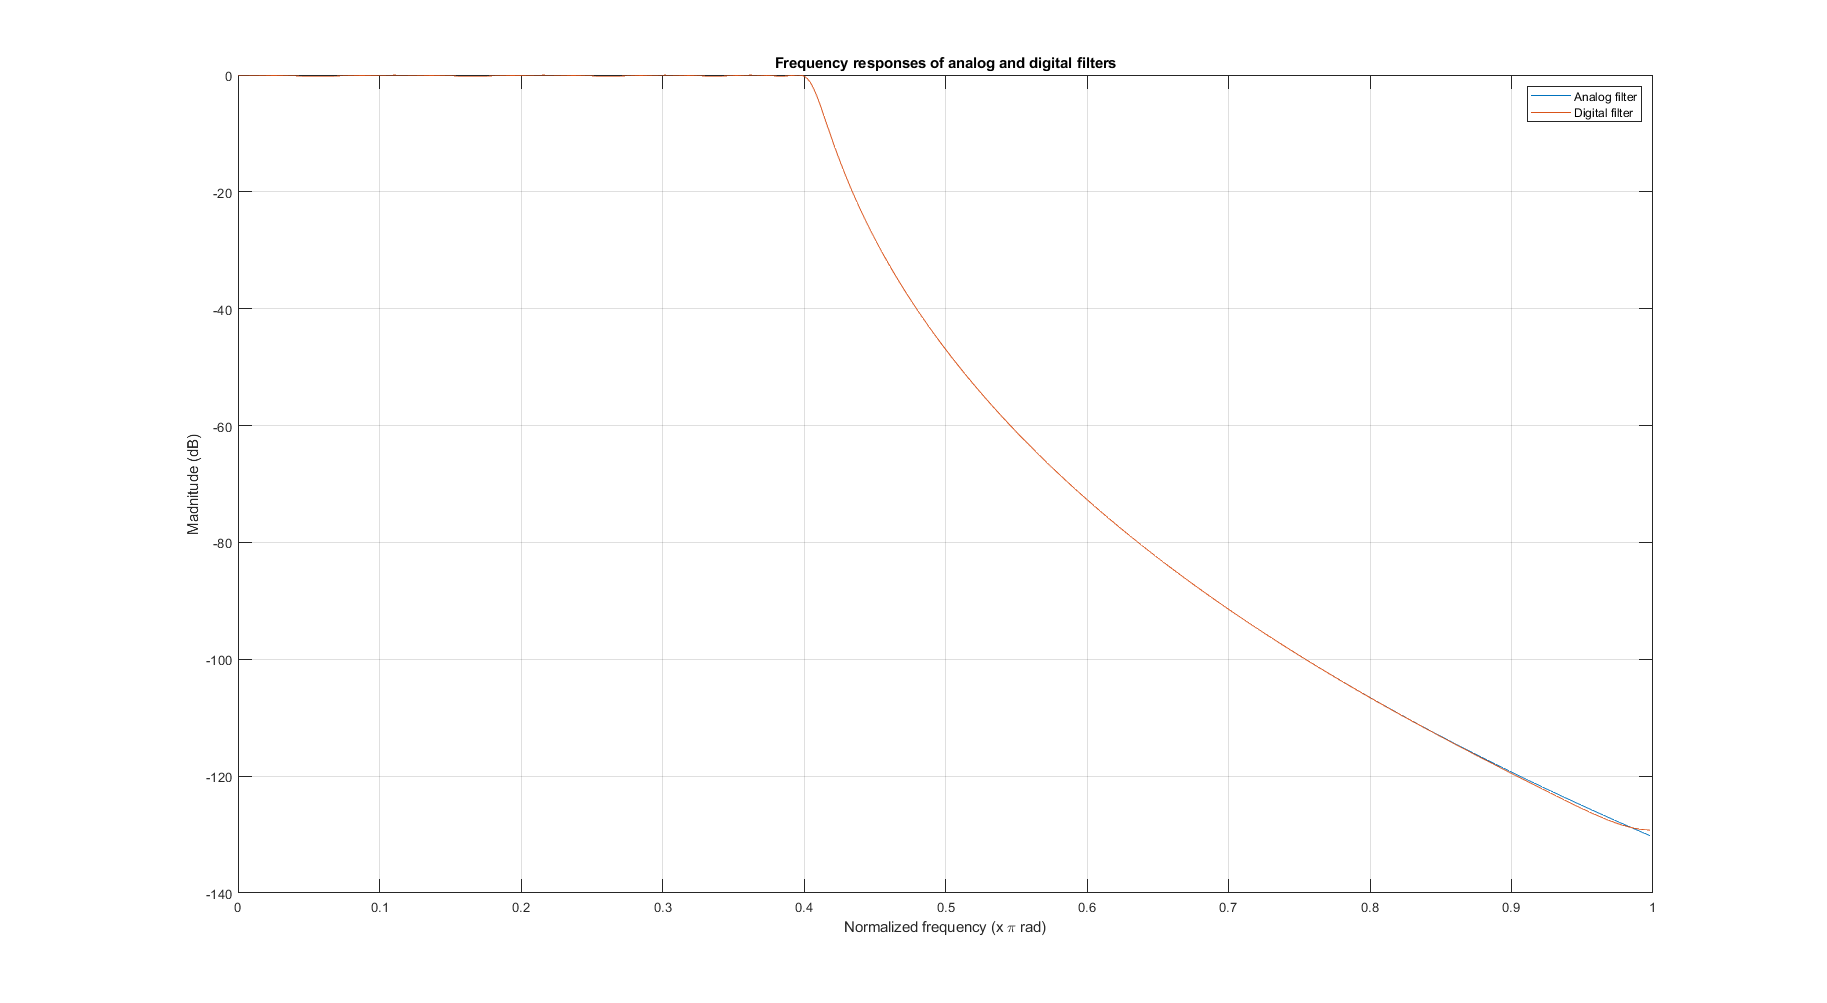
\includegraphics[scale=0.35]{Task2_FR.png}}
    \caption{Figure 5: Frequency response of the analog and the digital filters.}
    \label{fig:my_label}
\end{figure}
\newpage
\begin{lstlisting}
Fpass = 20e6;
Fstop = 25e6;
Fs = 100e6;
Ripple = 0.2;
Attenuation = 60;
Ws = 2 * Fstop / Fs; % normilize the frequency
Wp = 2 * Fpass / Fs; % normilize the frequency
[n, Wp] = cheb1ord(Wp, Ws, Ripple, Attenuation); % compute the order of 
% designing filter
[b,a] = cheby1(n, Ripple, 2 * pi * Fpass, 's'); % analog filter design B(s)/A(s)
figure(1);
[bz, az] = impinvar(b,a,Fs); % design a digital prototype of the analog 
% filter B(z)/A(z)
% the following steps are similar to the seminar
[r, p] = residue(b, a); % find direct term of a Partial Fraction Expansion of the
%ratio of two polynomials
t = linspace(0, 100 / Fs, 1000);
h = real(r.'*exp(p.*t) / Fs); % analog filter impulse response
plot(t, h)
hold on;
impz(bz, az, [], Fs); % digital filter impulse invariance
legend('Analog filter', 'Digital filter')
grid on;
hold off;

figure(2);
[H, W] = freqz(bz, az);
[H_an] = freqs(b, a, W * Fs);
H_dig_db = 20 * log10(abs(H)); % convert magnitude to dB
H_an_db = 20 * log10(abs(H_an));
plot(W / pi, H_an_db);
hold on;
plot(W / pi, H_dig_db);
legend('Analog filter', 'Digital filter')
title('Frequency responses of analog and digital filters')
ylabel('Madnitude (dB)')
xlabel('Normalized frequency (x \pi rad)')
grid on;
hold off;
\end{lstlisting}
According to the figure N!, digital filter approximates analog one with good accuracy.


\section*{Task 3}
Implement a digital prototype of the analog filter with the transfer function:
\begin{gather*}
    H(s) = \frac{s+2.5}{s^{2}+2.5s+4} 
\end{gather*}
using the Bilinear transformation. The sample clock frequency is Fs = 20 Hz. \\
a) Determine the linear Difference Equation of the digital filter.\\
b) Plot impulse and frequency responses for digital and analog filters. \\
Provide code. \\ \\
\textbf{Solution:}
Bilinear transformation equivalent to the substitution
\begin{gather*}
    s = \frac{2Fs(z-1)}{(z+1)}
\end{gather*}
the the transfer function of the analog filter $H(s)$
\begin{gather*}
    H(z) = \frac{\frac{2Fs(z-1)}{(z+1)} + 2.5}{(\frac{2Fs(z-1)}{(z+1)})^{2} + 2.5(\frac{2Fs(z-1)}{(z+1)}) + 4} 
    = \frac{2Fs(z-1) + 2.5(z+1)}{(z+1)(\frac{4Fs^{2}(z-1)^{2}}{(z+1)^{2}}) + 2.5(\frac{2Fs(z^2-1)}{(z+1)^2}) + \frac{4(z+1)^2}{(z+1)^2}} = \\
    = \frac{(z+1)(2Fs(z-1) + 2.5(z+1))}{4Fs^{2}(z-1)^{2}+5Fs(z^2-1)+4(z+1)^2} = \frac{(z+1)((2Fs+2.5)z+(2.5-2Fs))}{(4Fs^{2}+5Fs+4)z^{2}+(8-8Fs^{2})z+(4+4Fs^{2}-5Fs)} = \\
    =\frac{2Fs+2.5}{4Fs^{2}+5Fs+4}\frac{(z+1)(z+\frac{2.5-2Fs}{2Fs+2.5})}{z^2+\frac{8-8Fs^2}{4Fs^{2}+5Fs+4}z + \frac{4+4Fs^{2}-5Fs}{4Fs^{2}+5Fs+4}} = \frac{40+2.5}{1600+100+4}\frac{(z+1)(z+\frac{2.5-40}{40+2.5})}{z^2+\frac{8-3200}{1600+100+4}+\frac{4+1600-100}{1600+100+4}} = \\
    = 0.0249 \frac{(z+1)(z-0.8824)}{z^{2}-1.8732z+0.8826} = 
    0.0249 \frac{z^{2}(1+0.1176^{-1}+0.8824z^{-2})}{z^{2}(1-1.8732z^{-1}+0.8826z^{-2})} = \\
    =0.0249\frac{(1+0.1176^{-1}+0.8824z^{-2})}{(1-1.8732z^{-1}+0.8826z^{-2})} \\
    H(z) = \frac{Y(z)}{X(z)} = 0.0249\frac{(1+0.1176^{-1}+0.8824z^{-2})}{(1-1.8732z^{-1}+0.8826z^{-2})} \\
    0.0249X(z)(1+0.1176z^{-1}+0.8824z^{-2}) = Y(z)(1-1.8732z^{-1}+0.8826z^{-2}) \\
    X(z)(0.0249+0.0029z^{-1}+0.0220z^{-2}) = Y(z)(1-1.8732z^{-1}+0.8826z^{-2}) 
\end{gather*}
Using the time-shifting property I received the difference equation:
\begin{gather*}
    0.0249x[n]+0.0029x[n-1]+0.0220x[n-2] = y[n]-1.8732y[n-1]+0.8826y[n-2] 
\end{gather*}
Then I just wrote a simple Matlab code, which is similar to the code on seminar and plotted impulse and frequency responses for digital and analog filters.
\begin{figure}
    \begin{minipage}[h]{1\linewidth}
    \center{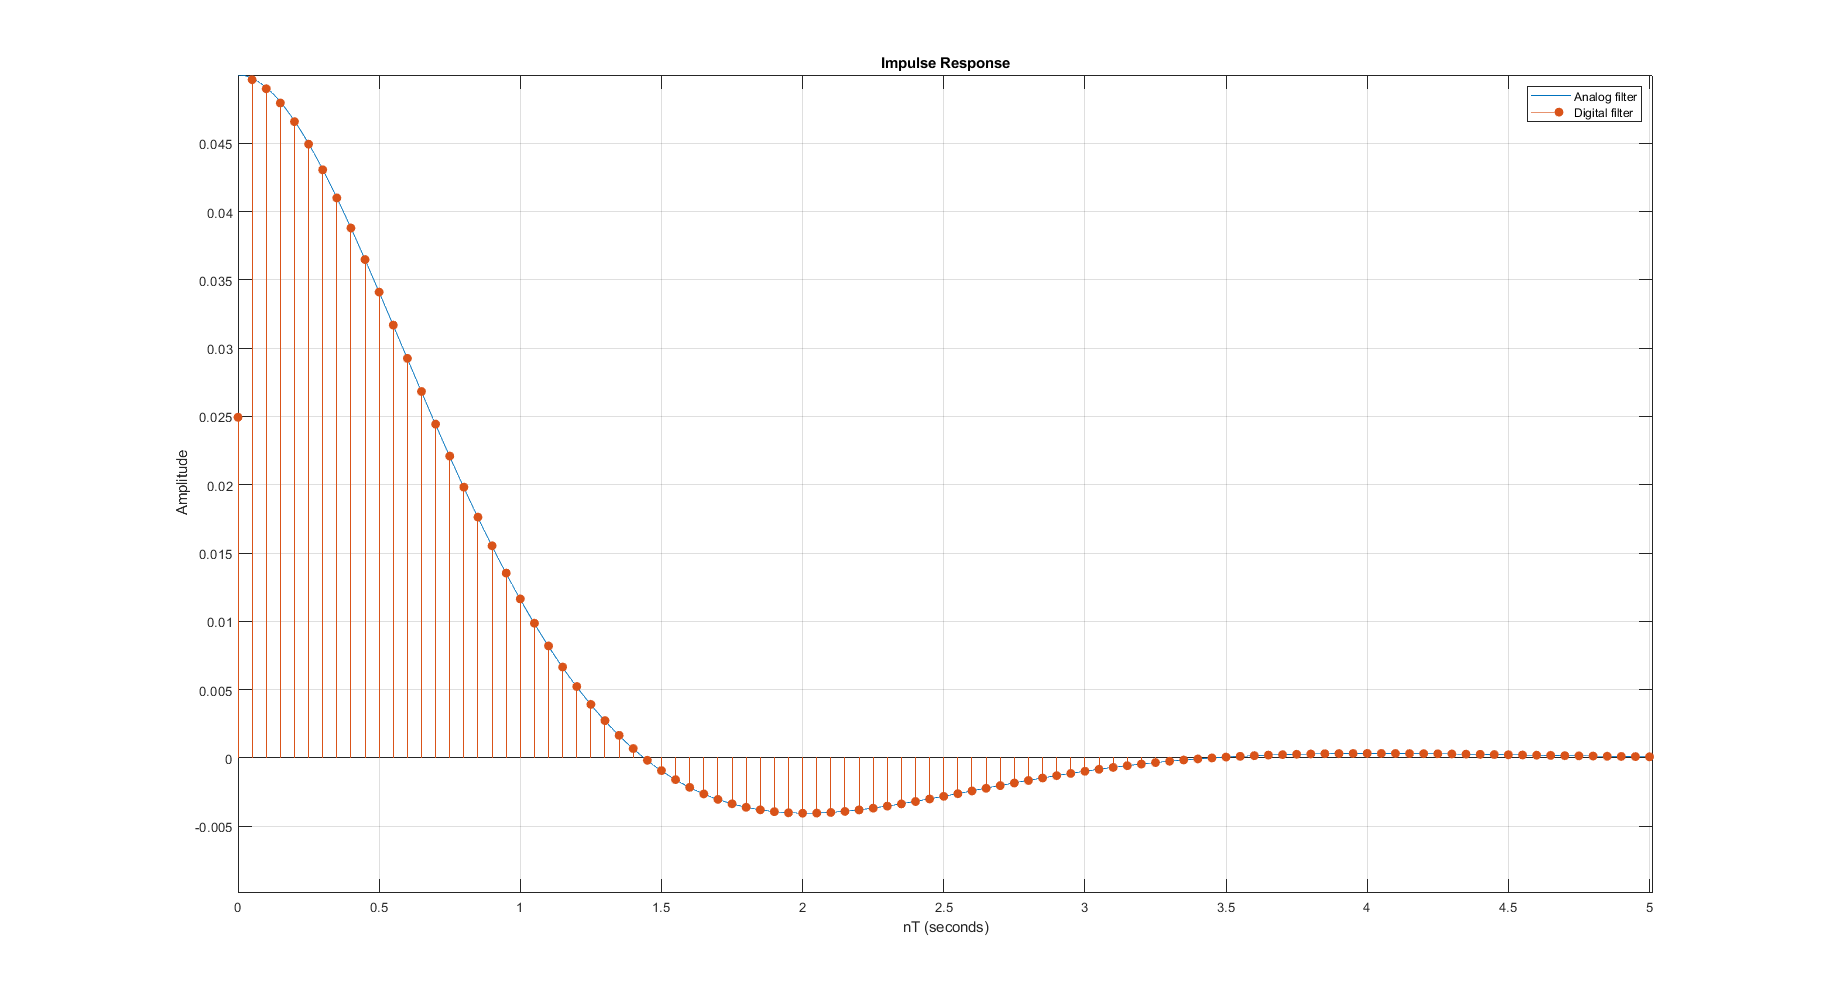
\includegraphics[scale=0.35]{Task3_IR.png}}
    \caption{Figure 6: Impulse response of the analog and the digital filters.}
    \label{fig:my_label}
    \end{minipage}
    \vfill
    \begin{minipage}[h]{1\linewidth}
    \center{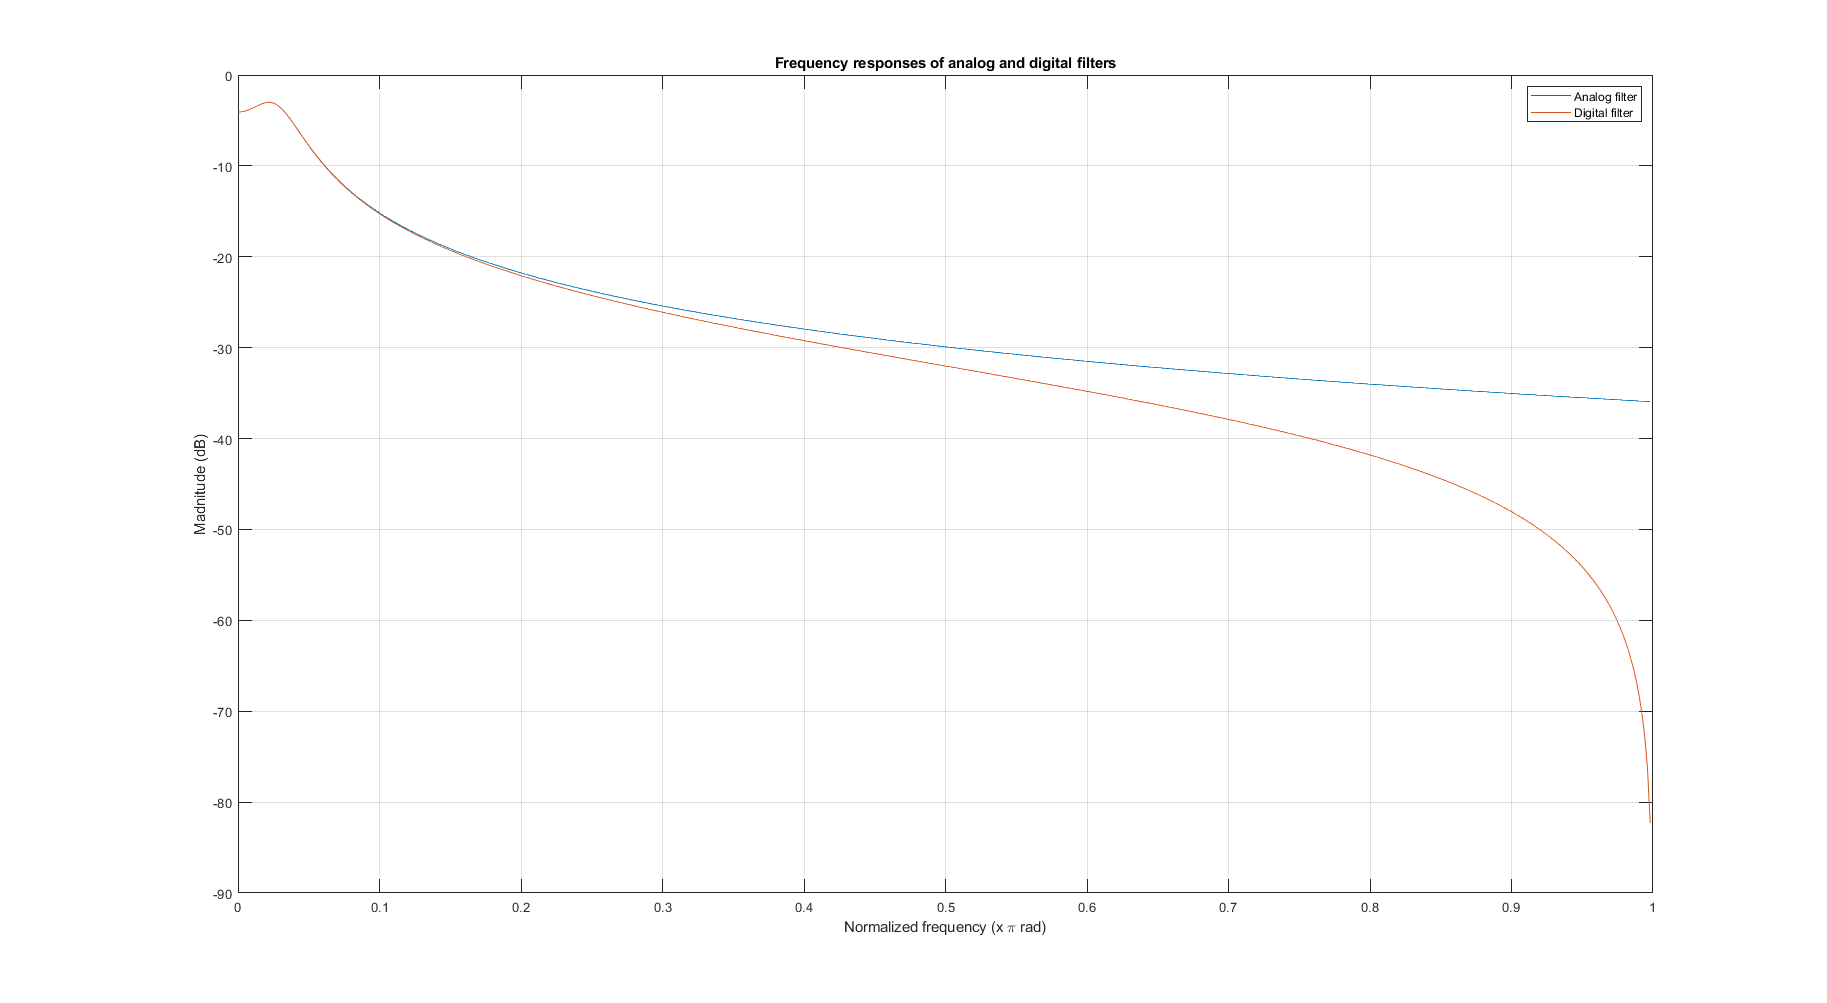
\includegraphics[scale=0.35]{Task3_FR.png}}
    \caption{Figure 7: Frequency response of the analog and the digital filters.}
    \label{fig:my_label}
    \end{minipage}
\end{figure}
\newpage
\begin{lstlisting}
Fs = 20;
b = [0 1 2.5];
a = [1 2.5 4];
[bz, az] = bilinear(b,a,Fs);
[r, p] = residue(b, a); % find direct term of a Partial Fraction Expansion of the 
%ratio of two polynomials
t = linspace(0, 100 / Fs, 1000);
h = real(r.'*exp(p.*t) / Fs); % analog filter impulse response
figure(1);
plot(t, h);
hold on;
impz(bz, az, [], Fs);
legend('Analog filter', 'Digital filter')
grid on;
hold off;

figure(2);
[H, W] = freqz(bz, az);
[H_an] = freqs(b, a, W * Fs);
H_dig_db = 20 * log10(abs(H)); % convert magnitude to dB
H_an_db = 20 * log10(abs(H_an));
plot(W / pi, H_an_db);
hold on;
plot(W / pi, H_dig_db);
legend('Analog filter', 'Digital filter')
title('Frequency responses of analog and digital filters')
ylabel('Madnitude (dB)')
xlabel('Normalized frequency (x \pi rad)')
grid on;
\end{lstlisting}
According to the figure with frequency response, digital prototype of the analog filter approximates the latter with good accuracy only when $f \leq 0.4Fs \rightarrow f \leq 8 MHz$.
\section*{Task 4}
A filter has the transfer function: 
$$ H(z) = 3+4z^{-1}+6z^{-2}+8z^{-3}$$
Determine the impulse response of the filter with the modified frequency response: 
$$ F(\omega) = H(\omega - \frac{\pi}{4}) $$
\textbf{Solution:} \\
First of all, let's move from Z-domain to frequency domain. For this substitute $z = re^{j\omega}$ to the expressions for the $H(z)$. Note: for simplicity I defined $r = 1$ so $z = e^{j\omega}$. I can do it, because $r$ is just a constant (like a scaling coefficient for each summond). \\
$$H(\omega) = 3 + 4e^{-j\omega} + 6e^{-j2\omega} + 8e^{-j3\omega}$$
Then for our task substitute modified frequency: $\omega^{*} = \omega -\frac{\pi}{4}$
$$H(\omega) = 3 + 4e^{-j(\omega - \frac{\pi}{4})} + 6e^{-j(2\omega -\frac{\pi}{2})} + 8e^{-j(3\omega-\frac{3\pi}{4})} $$
$$H(\omega) = 3 + 4e^{\frac{j\pi}{4}}e^{-j\omega}+6e^{\frac{j\pi}{2}}e^{-j2\omega}+8e^{\frac{j3\pi}{4}}e^{-j3\omega}$$
So then I need to calculate inverse DTFT:
\begin{gather*}
    h[n] = \frac{1}{2\pi}\int_{-\pi}^{\pi}{H(\omega)e^{j\omega n}d\omega}\\
    h[n] = \frac{1}{2\pi}\int_{-\pi}^{\pi}{(3+4e^{\frac{j\pi}{4}}e^{-j\omega} + 6e^{\frac{j\pi}{2}}e^{-j2\omega} +8e^{\frac{j3\pi}{4}}e^{-j3\omega})e^{j\omega n}d\omega}\\
    h[n] = \frac{1}{2\pi}\int_{-\pi}^{\pi}{(3e^{j\omegan}+4e^{\frac{j\pi}{4}}e^{j\omega(n-1)}+6e^{\frac{j\pi}{2}}e^{j\omega(n-2)}+8e^{\frac{j3\pi}{4}}e^{j\omega (n-3)})} d \omega\\
    h[n] = \frac{1}{2\pi}(\frac{3}{jn}e^{j\omega n }|_{-\pi}^{\pi}+4e^{\frac{j\pi}{4}}\frac{e^{j\omega (n-1)}}{j(n-1)}|_{-\pi}^{\pi} + 6e^{\frac{j\pi}{2}}\frac{e^{j\omega(n-2)}}{j(n-2)}|_{-\pi}^{\pi} + 8e^{\frac{j3\pi}{4}}\frac{e^{j\omega(n-3)}}{j(n-3)}|_{-\pi}^{\pi})\\
    h[n] = \frac{1}{2\pi}(\frac{6}{n}(\frac{e^{j\pi n} - e^{-j\pi n}}{2 j}) + \frac{8e^{\frac{j\pi}{4}}}{n-1}(\frac{e^{j\pi(n-1)}-e^{-j\pi(n-1)}}{2j})+ \frac{12e^{\frac{j\pi}{2}}}{n-2}(\frac{e^{j\pi(n-2)}-e^{-j\pi(n-2)}}{2j})+\\
    +\frac{16e^{\frac{j3\pi}{4}}}{n-3}(\frac{e^{j\pi(n-3)}-e^{-j\pi(n-3)}}{2j})\\
    h[n]=\frac{3sin(\pi n)}{\pi n} + \frac{4e^{\frac{j\pi}{4}}sin(\pi(n-1))}{\pi(n-1)} + \frac{6e^{\frac{j\pi}{2}}sin(\pi(n-2))}{\pi(n-2)} + 
    \frac{8e^{\frac{j3\pi}{4}}sin(\pi(n-3))}{\pi(n-3)}\\
    h[n] = 3\delta[n] + 4e^{\frac{j\pi}{4}}\delta[n-1]+6e^{\frac{j\pi}{2}}\delta[n-2]+ 8e^{\frac{j 3 \pi}{4}}\delta[n-3]\\
\end{gather*}
\[   
h[n] = 
     \begin{cases}
       3 & ,n = 0\\
       4e^{\frac{j\pi}{4}} &, n = 1\\
       6e^{\frac{j\pi}{2}} &, n = 2\\
       8e^{\frac{3j\pi}{4}} &, n = 3\\
       0 &, \text{otherwise}
     \end{cases}
\]
\section*{Task 5}
For a linear system with the transfer function:
\begin{gather*}
    H(z) = \frac{1z+2}{3z^{3}  + 4z^{2} + 5z+ 6}
\end{gather*}
a) Calculate the difference equation relating the input x[n] to the output y[n]. \\
b) Design block diagram realization (Direct-Form 1 and Direct-Form 2). \\
c) Plot impulse and frequency responses. \\ \\
\textbf{Solution:} \\
\begin{gather*}
    H(z) = \frac{Y(z)}{X(z)} = \frac{1z+2}{3z^{3}  + 4z^{2} + 5z+ 6} = \frac{z^{3}(z^{-2}+2z^{-3})}{z^{3}(3+4z^{-1}+5z^{-2}+6z^{-3})} \\
    X(z)(z^{-2}+2z^{-3}) = Y(z)(3+4z^{-1}+5z^{-2}+6z^{-3})
\end{gather*}
Using the time-shifting property I received the difference equation:
\begin{gather*}
    x[n-2]+2x[x-3] = 3y[n]+4y[n-1]+5y[n-2]+6y[n-3] \\
    y[n] = \frac{1}{3}x[n-2]+\frac{2}{3}x[n-3]-\frac{4}{3}y[n-1]-\frac{5}{3}y[n-2]-2y[n-3]
\end{gather*}
Then I designed block diagram realization in Direct-Form I and Direct-Form II:
\begin{figure}
    \begin{minipage}[h]{1\linewidth}
    \center{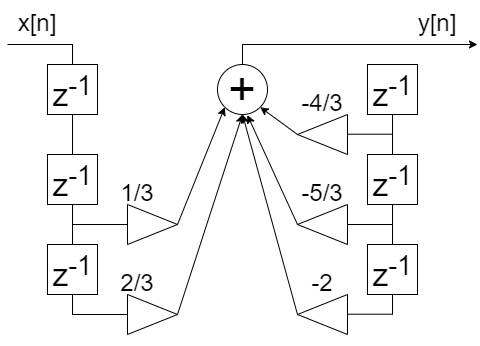
\includegraphics[scale=1]{Task5_DF1.png}}
    \caption{Figure 8: Direct-Form I.}
    \label{fig:my_label}
    \end{minipage}
    \vfill
    \begin{minipage}[h]{1\linewidth}
    \center{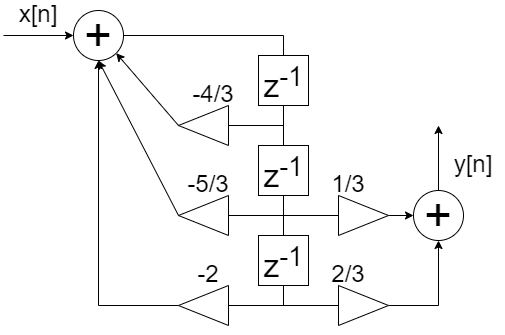
\includegraphics[scale=1]{Task5_DF2.png}}
    \caption{Figure 9: Direct-Form II.}
    \label{fig:my_label}
    \end{minipage}
\end{figure}
And then I plotted impulse and frequency responses for this linear system:
\begin{figure}
    \begin{minipage}[h]{1\linewidth}
    \center{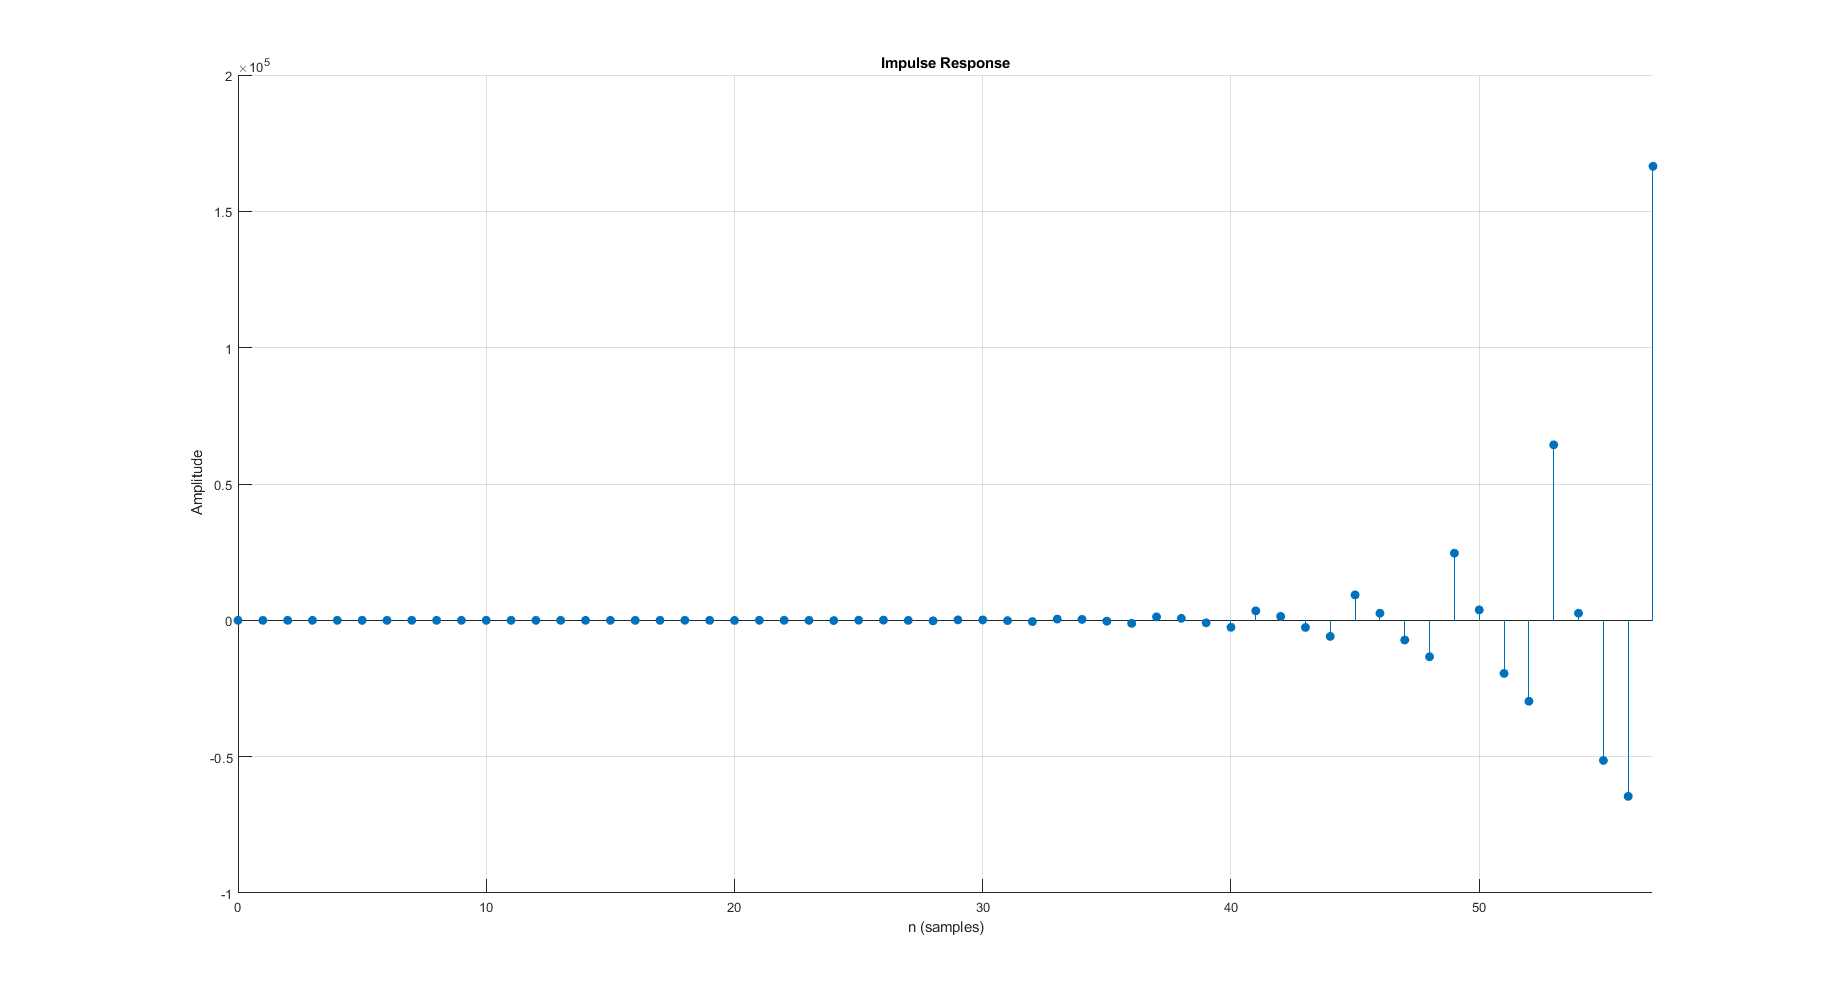
\includegraphics[scale=0.35]{Task5_IR.png}}
    \caption{Figure 10: Impulse response of the linear system.}
    \label{fig:my_label}
    \end{minipage}
    \vfill
    \begin{minipage}[h]{1\linewidth}
    \center{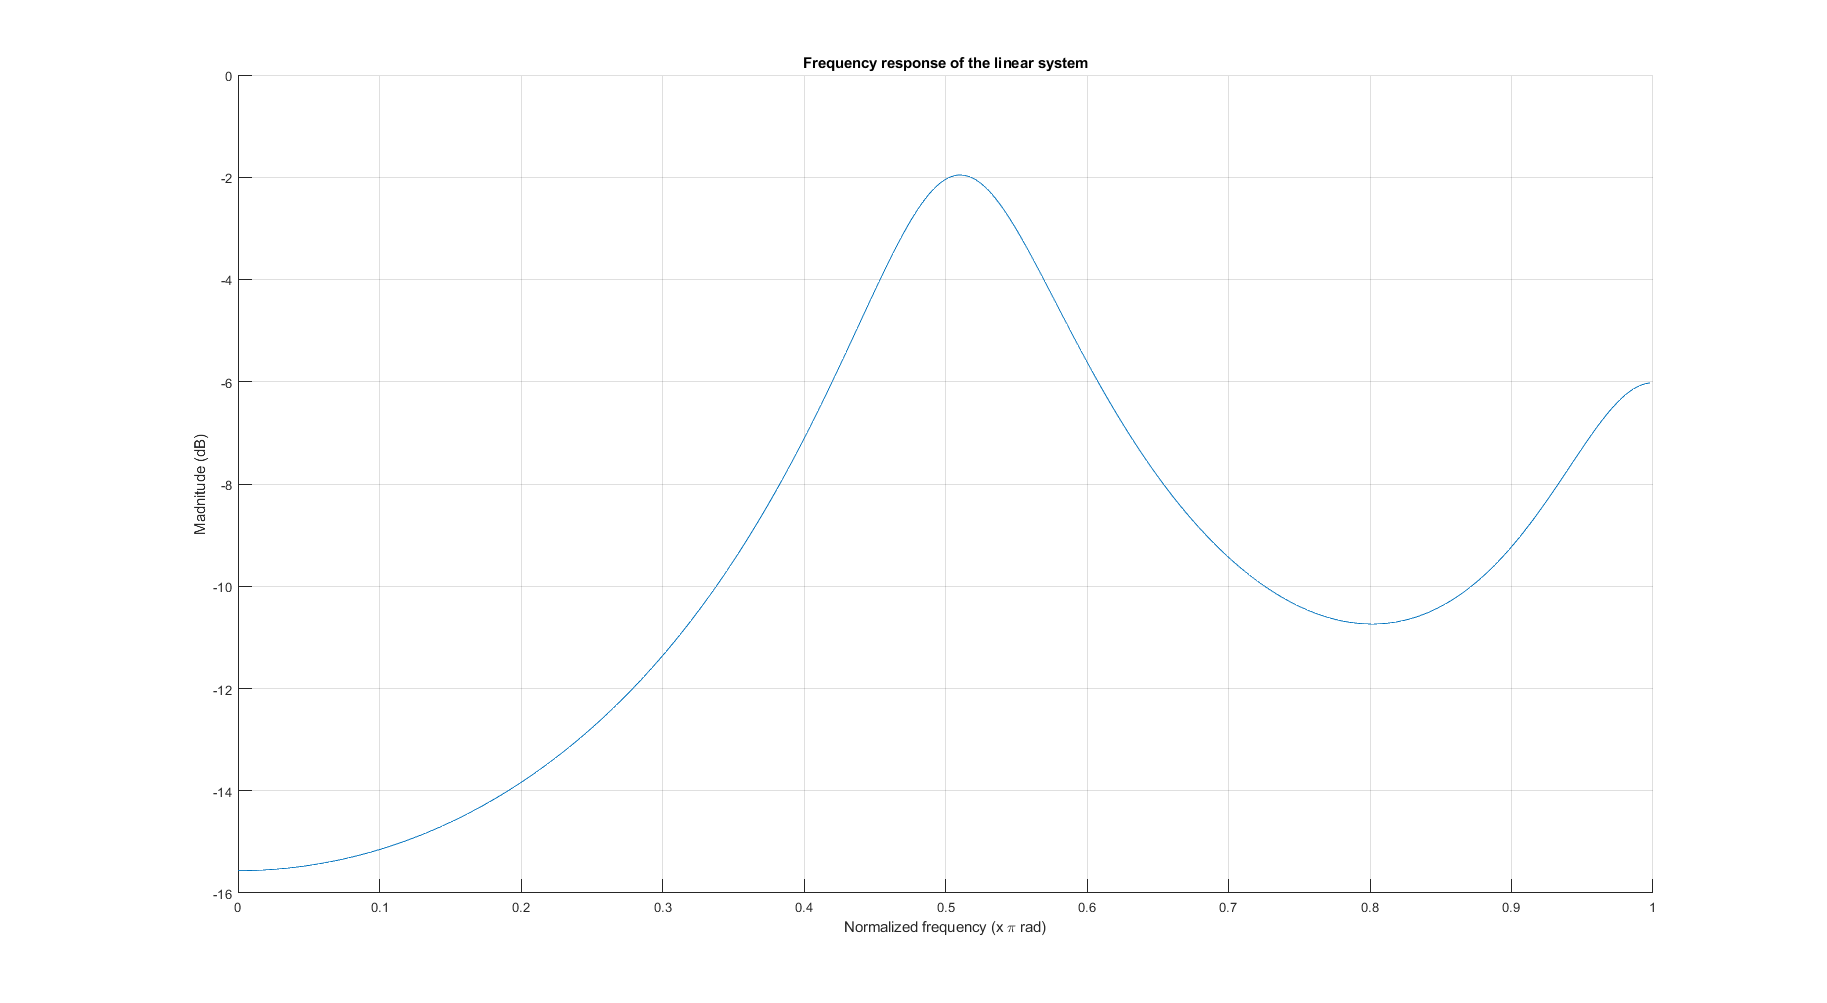
\includegraphics[scale=0.35]{Task5_FR.png}}
    \caption{Figure 11: Frequency response of the linear system.}
    \label{fig:my_label}
    \end{minipage}
\end{figure}
\newpage
\begin{lstlisting}
bz = [0 0 1 2];
az = [3 4 5 6];

figure(1);
hold on;
impz(bz, az);
grid on;
hold off;

figure(2);
[H, W] = freqz(bz, az);
H_dig_db = 20 * log10(abs(H)); % convert magnitude to dB
hold on;
plot(W / pi, H_dig_db);
title('Frequency response of the linear system')
ylabel('Madnitude (dB)')
xlabel('Normalized frequency (x \pi rad)')
grid on;
hold off;


\end{lstlisting}

\end{document}
